\documentclass[tikz,border=8pt]{standalone}
\usepackage{amsmath}
\usepackage{amssymb}
\usetikzlibrary{arrows.meta,patterns}

\definecolor{insideblue}{RGB}{31,104,157}
\definecolor{entrygreen}{RGB}{66,135,96}
\definecolor{outsideorange}{RGB}{181,92,41}
\definecolor{softgray}{RGB}{86,86,86}
\definecolor{paleintensive}{RGB}{209,230,245}
\definecolor{paleentry}{RGB}{245,220,198}
\definecolor{postfill}{RGB}{222,238,226}

\begin{document}
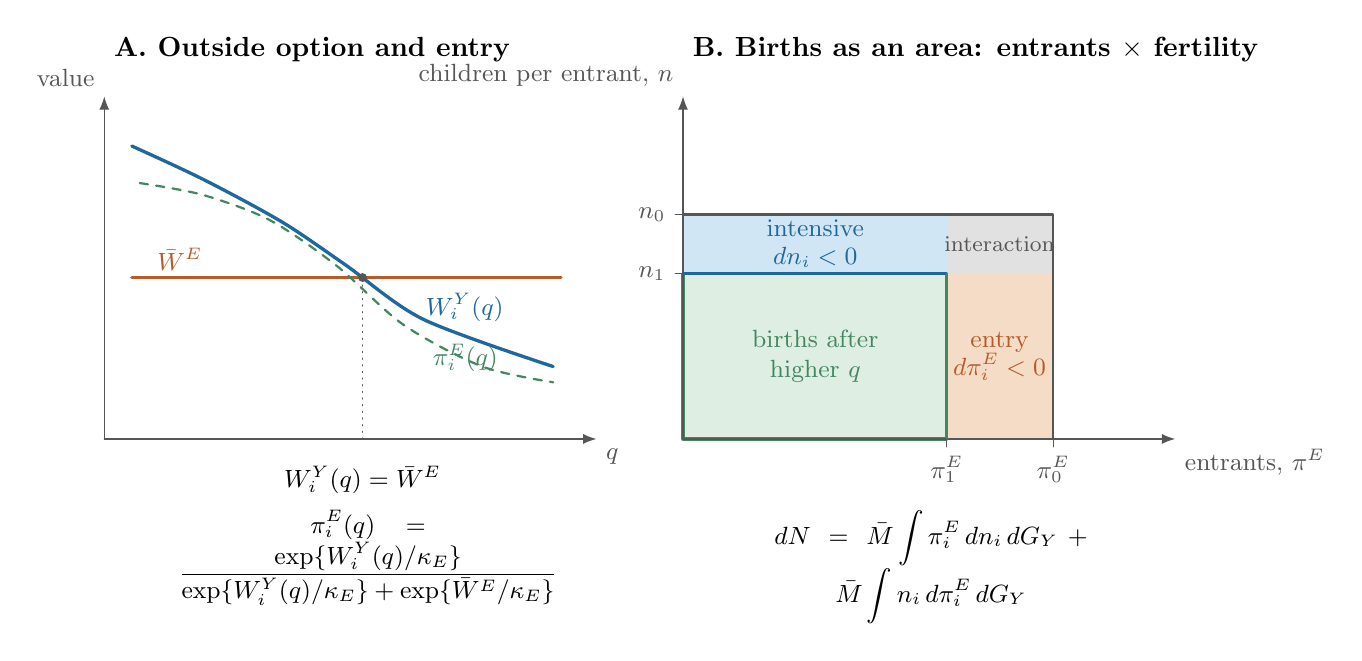
\begin{tikzpicture}[font=\small, >=Latex, line cap=round, line join=round]

% ---------- Panel A ----------
\begin{scope}[shift={(0,0)}]
  \node[anchor=west,font=\bfseries] at (0,4.95) {A. Outside option and entry};
  \draw[->,softgray] (0,0) -- (6.25,0) node[below right] {$q$};
  \draw[->,softgray] (0,0) -- (0,4.35) node[above left] {value};

  \draw[insideblue,very thick,smooth]
    plot coordinates {(0.35,3.72) (1.25,3.30) (2.25,2.76) (3.05,2.22) (4.05,1.52) (5.70,0.92)};
  \draw[outsideorange,very thick] (0.35,2.05) -- (5.80,2.05);
  \draw[softgray,dotted] (3.28,0) -- (3.28,2.05);
  \fill[softgray] (3.28,2.05) circle (1.6pt);

  \draw[entrygreen,thick,dashed,smooth]
    plot coordinates {(0.45,3.25) (1.25,3.10) (2.10,2.78) (2.95,2.20) (3.80,1.45) (4.80,0.92) (5.70,0.72)};
  \node[entrygreen,anchor=west] at (4.05,1.03) {$\pi_i^E(q)$};
  \node[insideblue,anchor=west] at (3.96,1.67) {$W_i^Y(q)$};
  \node[outsideorange,anchor=west] at (0.55,2.28) {$\bar W^E$};
  \node[align=center,anchor=north] at (3.28,-0.22) {$W_i^Y(q)=\bar W^E$};

  \node[align=center,anchor=north west,text width=5.75cm] at (0.35,-0.78)
    {$\displaystyle
    \pi_i^E(q)=
    \frac{\exp\{W_i^Y(q)/\kappa_E\}}
    {\exp\{W_i^Y(q)/\kappa_E\}+\exp\{\bar W^E/\kappa_E\}}$};
\end{scope}

% ---------- Panel B ----------
\begin{scope}[shift={(7.35,0)}]
  \node[anchor=west,font=\bfseries] at (0,4.95) {B. Births as an area: entrants $\times$ fertility};
  \draw[->,softgray] (0,0) -- (6.25,0) node[below right] {entrants, $\pi^E$};
  \draw[->,softgray] (0,0) -- (0,4.35) node[above left] {children per entrant, $n$};

  \fill[postfill] (0,0) rectangle (3.35,2.10);
  \draw[entrygreen,very thick] (0,0) rectangle (3.35,2.10);
  \fill[paleintensive] (0,2.10) rectangle (3.35,2.85);
  \fill[paleentry] (3.35,0) rectangle (4.70,2.10);
  \fill[softgray!18] (3.35,2.10) rectangle (4.70,2.85);
  \draw[softgray,thick] (0,0) rectangle (4.70,2.85);

  \draw[insideblue,thick] (0,2.10) -- (3.35,2.10);
  \draw[entrygreen,thick] (3.35,0) -- (3.35,2.10);

  \node[align=center,insideblue] at (1.68,2.48)
    {intensive\\[-1pt] $dn_i<0$};
  \node[align=center,outsideorange] at (4.02,1.05)
    {entry\\[-1pt] $d\pi_i^E<0$};
  \node[align=center,entrygreen] at (1.68,1.05)
    {births after\\higher $q$};
  \node[align=center,softgray] at (4.02,2.48)
    {\footnotesize interaction};

  \draw[softgray,dashed] (0,2.85) -- (-0.10,2.85) node[left] {$n_0$};
  \draw[softgray,dashed] (0,2.10) -- (-0.10,2.10) node[left] {$n_1$};
  \draw[softgray,dashed] (4.70,0) -- (4.70,-0.10) node[below] {$\pi_0^E$};
  \draw[softgray,dashed] (3.35,0) -- (3.35,-0.10) node[below] {$\pi_1^E$};

  \node[align=center,anchor=north west,text width=5.95cm] at (0.05,-0.78)
    {$\displaystyle
    dN=\bar M\int \pi_i^E\,dn_i\,dG_Y
      +\bar M\int n_i\,d\pi_i^E\,dG_Y$};
\end{scope}

\end{tikzpicture}
\end{document}
